\section{Introduction}

To recognize context-free languages, an automaton with an auxiliary component structured as an unbounded stack of symbols is necessary. 
The stack operations include:
\begin{itemize}
    \item \textit{Push}: adds the symbol(s) onto the top of the stack.
    \item \textit{Pop}: removes the symbol from the top of the stack if it's not empty; otherwise, reads $Z_0$.
    \item \textit{Stack emptiness test}: returns true if the stack is empty, and false otherwise.
\end{itemize}
The symbol $Z_0$ represents the stack bottom and can be read but not removed. 
Additionally, the symbol $\dashv$ serves as the terminator character for the input string.
The configuration is determined by the current state, current character, and stack contents. 
During a move, the pushdown automaton:
\begin{itemize}
    \item Reads the current character, shifting the input head or performing a spontaneous move without shifting the input head.
    \item Reads the stack's top symbol, removing it if the stack is not empty, or reading the stack symbol $Z_0$ if the stack is empty.
    \item Depending on the current character, state, and stack top symbol, transitions into the next state and places none, one, or more symbols onto the top of the stack.
\end{itemize}

\paragraph*{Pushdown automaton}
A pushdown automaton $M$ is defined by:
\begin{itemize}
    \item $Q$: a finite set of states for the control unit.
    \item $\Sigma$: a finite input alphabet.
    \item $\Gamma$: a finite stack alphabet.
    \item $\delta$: a transition function.
    \item $q_0 \in Q$: the initial state.
    \item $Z_0 \in \Gamma$: the initial stack symbol.
    \item $F \subseteq Q$: a set of final states.
\end{itemize}
The transition function $\delta$ is defined as follows:
\begin{itemize}
    \item \textit{Domain}: $Q \times \left(\Sigma \cup \{\varepsilon\}\right) \times \Gamma$. 
    \item \textit{Image}: the set of the subsets of $Q \times \Gamma^{*}$. 
\end{itemize}
Possible moves include:
\begin{itemize}
    \item \textit{Reading move}: in state $q$ with symbol $Z_0$ on the top of the stack, the automaton reads the character $a$ and transitions to one of the states $p_i$ (where $1 \leq i \leq n$), after sequentially performing pop and push operations ($\gamma_i$): 
        \[\delta(q,a,Z)=\{(p_1,\gamma_1), (p_2,\gamma_2),\dots,(p_n,\gamma_n)\}\]
    \item \textit{Spontaneous move}: n state $q$ with symbol $Z_0$ on the top of the stack, the automaton does not read any input character and transitions to one of the states $p_i$ (where $1 \leq i \leq n$), after sequentially executing pop and push operations ($\gamma_i$):
        \[\delta(q,\varepsilon,Z)=\{(p1,\gamma_1), (p2,\gamma_2),\dots,(p_n,\gamma_n)\}\]
\end{itemize}
\begin{table}[H]
    \centering
    \begin{tabular}{ccc}
    \hline
    \textbf{Current configuration} & \textbf{Next configuration} & \textbf{Applied move} \\ \hline
    $(q,az,\eta Z)$                & $(p,z,\eta\gamma)$          & Reading               \\
    $(q,az,\eta Z)$                & $(p,az,\eta\gamma)$         & Spontaneous           \\ \hline
    \end{tabular}
\end{table}

\paragraph*{Pushdown automaton configurations}
Non-determinism arises when considering a triple (state, input, stack top), as there exist two or more potential moves that involve consuming either none or one input character.
\begin{definition}[\textit{Instantaneous configuration}]
    The instantaneous configuration of a machine $M$ is a 3-tuple: 
    \[(q,y,\eta)\in Q \times \Sigma^{*} \times \Gamma^{+}\]
\end{definition}
Here, $q$ is the current state of the control unit, $y$ is the part of the input string $x$ that still has to be scanned, and $\eta$ is the current contents of the pushdown stack.
\begin{definition}[\textit{Initial configuration}]
    The \emph{initial} configuration of machine $M$ is: 
    \[(q_0,x,Z_0)\]
\end{definition}
\begin{definition}[\textit{Final configuration}]
    The \emph{final} configuration of machine $M$ is: 
    \[(q,\varepsilon,\lambda)\]
\end{definition}

Executing a move results in a transition from one configuration to another, represented as:
\[(q,y,\eta)\rightarrow(p,z,\lambda)\]
It is important to note that a sequence of one or more transitions is denoted by $\overset{+}{\rightarrow}$. 

An input string $x$ is deemed accepted by a final state if the following computation exists:
\[(q_0,x,Z_0)\overset{*}{\mapsto}(q,\varepsilon,\lambda)\]
Here, $q \in F$ and $\lambda\in\Gamma^{*}$. 
It is worth mentioning that there is no specific condition for $\lambda$; sometimes it may be the empty string, but this is not a mandatory requirement.

\subsection{State-transition graph}
The transition function of a finite automaton can be visually depicted. 
The numerator of the representation denotes the characters read from the input tape and the memory. 
Meanwhile, the denominator indicates the replacement for the element in the stack memory.
\begin{example}
    The language $L=\{uu^R|u \in \{a,b\}^{*}\}$, consisting of palindromes of even length, is recognized with a final state by the pushdown recognizer. 
    The graphical representation is illustrated in the following figure:
    \begin{figure}[H]
        \centering
        \includegraphics[width=0.6\linewidth]{images/pda.png}
    \end{figure}
\end{example}

\subsection{From grammar to pushdown automata}
Grammar rules can be interpreted as the instructions for a nondeterministic pushdown automaton, which operates in a goal-oriented manner, utilizing the stack as a notebook for the sequence of upcoming actions.

The stack symbols in this automaton can represent both terminals and non-terminals from the grammar.
If the stack contains the symbol sequence $A_1 \dots A_k$, the automaton first executes the action associated with $A_k$. 
This action aims to determine, from the current position $a_i$ in the input string, if there exists a string $w$ derivable from $A_k$.
If so, the action shifts the input head by $\left\lvert w\right\rvert$ positions.

An action may recursively break down into a series of sub-actions, especially when recognizing the non-terminal symbol $A_k$ requires recognizing other non-terminals.

The initial action corresponds to the grammar axiom: the pushdown recognizer checks whether the source string can be derived from the axiom.
Initially, the stack contains only the symbol $Z_0$ and the axiom $S$, and the input head is positioned at the beginning of the input string.
At each step, the automaton nondeterministically chooses an applicable grammar rule and performs the corresponding move.
The input string is considered accepted only when it has been entirely scanned and the stack is empty.

Given a grammar $G=(V,\Sigma,P,S)$ with $A,B \in V$, $b \in \Sigma$ and $A_i \in V \cup \Sigma$, the correspondence between a grammar and a pushdown automaton is summarized as follows: 
\begin{table}[H]
    \centering
    \begin{tabular}{|cc|}
    \hline
    \textbf{Grammar rule}                                      & \textbf{Automaton move}                                                                                    \\ \hline
    $A \rightarrow B A_1\dots A_n \textnormal{ with }n \geq 0$ & \makecell{If $\textnormal{top}=A$ then pop \\ Push $(A_n \dots A_1B)$}                                     \\ \hline
    $A \rightarrow b A_1\dots A_n \textnormal{ with }n \geq 0$ & \makecell{If $cc=b$ and $\textnormal{top}=A$ then pop \\ Push $(A_n \dots A_1)$ \\ Shift reading head}     \\ \hline
    $A \rightarrow \varepsilon$                                & If $\textnormal{top}=A$ then pop                                                                           \\ \hline
    For every character $b \in \Sigma$                         & \makecell{If $cc=b$ and $\textnormal{top}=b$ then pop \\ Shift reading head}                               \\ \hline
    ---                                                        & \makecell{If $cc=\dashv$ and the stack is empty then accept \\ Halt}                                       \\ \hline
    \end{tabular}
\end{table}
\begin{example}
    Consider the language $L=\{a^nb^m|n \geq m \geq 1\}$, the corresponding nondeterministic grammar generating strings of this language is presented below:
    \[\begin{cases}
        S \rightarrow aS \\
        S \rightarrow A \\
        A \rightarrow aAb \\
        A \rightarrow ab
    \end{cases}\]
    Utilizing the rules from the previous table, we can construct the pushdown automaton as depicted in the following:
    \begin{table}[H]
        \centering
        \begin{tabular}{ccc}
        \hline
        $\#$ & \textbf{Grammar rule}    & \textbf{Automaton move}                                                                                   \\ \hline
        1    & $ S \rightarrow aS$      & \makecell{If $cc=a$ and $\textnormal{top}=S$ then pop \\ Push $S$ \\ Shift reading head}                  \\ 
        2    & $S \rightarrow A$        & \makecell{If $\textnormal{top}=S$ then pop \\ Push$(A)$   }                                               \\ 
        3    & $A \rightarrow aAb$      & \makecell{If $cc=a$ and $\textnormal{top}=A$ then pop \\ Push $bA$ \\ Shift reading head}                 \\ 
        4    & $A \rightarrow ab$       & \makecell{If $cc=a$ and $\textnormal{top}=A$ then pop \\ Push $b$ \\ Shift reading head}                  \\ 
        5    & ---                      & \makecell{If $cc=b$ and $\textnormal{top}=b$ then pop \\ Shift reading head}                              \\ 
        6    & ---                      & \makecell{If $cc=\dashv$ and the stack is empty then accept \\ Halt}                                      \\ \hline
        \end{tabular}
    \end{table}
\end{example}
The automaton recognizes a string if and only if the string is generated by the grammar; each successful automaton computation corresponds to a grammar derivation, and vice versa.
Therefore, the automaton simulates the leftmost derivations of the grammar.
However, the automaton lacks the ability to guess the correct derivation; it must explore all possibilities.
A string is accepted by two or more different computations if and only if the grammar is ambiguous.

\paragraph*{Reverse transformation}
The process of constructing an automaton from grammar can be reversed, yielding the grammar by starting from the pushdown automaton, provided it is a one-state automaton.
\begin{property}
    The family of free languages generated by free grammars is identical to the family of languages recognized by one-state pushdown automata.
\end{property}
Unfortunately, in general, the resulting pushdown automaton is nondeterministic, as it explores all applicable moves at any point and exhibits an exponential time complexity concerning the length of the source string.

\subsection{Varieties of pushdown automata}
There are three acceptance modes for pushdown automata:
\begin{enumerate}
    \item \textit{By final state}: accepts when it enters a final state regardless of the stack contents.
    \item \textit{By empty stack}: accepts when the stack becomes empty regardless of the current state.
    \item \textit{Combined}: accepts by both final state and empty stack.
\end{enumerate}
\begin{property}
    For the family of nondeterministic pushdown automata with states, the three acceptance modes mentioned above are equivalent.
\end{property}
A generic pushdown automaton may perform an unlimited number of moves without reading any input character, but only if it enters a loop consisting only of spontaneous moves.
This behavior either prevents it from fully reading the input string or causes it to execute an unlimited number of moves before deciding to accept or reject the string.
Both of these behaviors are undesirable in practice. 
However, it is always possible to construct an equivalent automaton without spontaneous loops.

\paragraph*{On-line mode}
A pushdown automaton operates in an on-line mode if it decides to accept or reject the string as soon as it reads the last character of the input string and does not execute any further moves. 
From a practical perspective, the on-line mode is desirable. 
It is always feasible to build an equivalent automaton that operates in an on-line mode.

\subsection{Context-free languages and pushdown automata}
The language accepted by a generic pushdown automaton is context free. 
Moreover, any free language can be recognized by a nondeterministic one-state pushdown automaton.
\begin{property}
    The family CF of context-free languages is equivalent to the set of languages recognized by unrestricted pushdown automata.
\end{property}
\begin{property}
    The family CF of context-free languages is identical to the set of languages recognized by nondeterministic one-state pushdown automata.
\end{property}

\subsection{Intersection of regular and context-free languages}
It can be easily demonstrated that the intersection of a context free and a regular language is also context free.
To recognize the intersection$L(G) \cap L(A)$ where $G$ is a grammar and $A$ is a finite state automaton, the pushdown automaton $M$ can be obtained as follows: 
\begin{enumerate}
    \item Construct a one-state pushdown automaton $N$ that recognizes $L (G)$ by empty stack. 
    \item Build the pushdown automaton $M$ whose state-transition graph is the Cartesian product of the state-transition graphs of $N$ and $A$ using the Cartesian product construction.
        Ensure that the actions of $M$ on the stack are the same as those of $N$. 
\end{enumerate}
The resulting pushdown automaton $M$: 
\begin{enumerate}
    \item Has pairs of states from the component machines $N$ and $A$ as its states. 
    \item Accepts by the combined acceptance mode of final state and empty stack.
    \item Consider states containing a final state of $A$ as final states.
    \item Is deterministic if both component machines $N$ and $A$ are deterministic.
    \item Accepts by final state all and only the strings belonging to the intersection language.
\end{enumerate}
\begin{example}
    Consider the Dyck language $L=\{a^na^{'n}| n \geq 1\}$. 
    A finite state automaton that recognizes the language by final state can be constructed as follows:
    \begin{figure}[H]
        \centering
        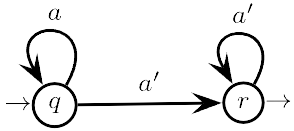
\includegraphics[width=0.3\linewidth]{images/pdaint.png}
    \end{figure}
    Additionally, a pushdown automaton that recognizes the language by empty stack can be constructed as follows:
    \begin{figure}[H]
        \centering
        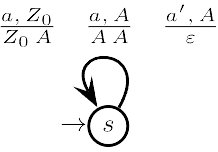
\includegraphics[width=0.25\linewidth]{images/pdaint1.png}
    \end{figure}
    Applying the intersection, we obtain a product pushdown automaton that recognizes by empty stack in the final state $(r,s)$: 
    \begin{figure}[H]
        \centering
        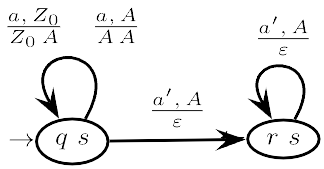
\includegraphics[width=0.3\linewidth]{images/pdaint2.png}
    \end{figure}
\end{example}